% Sample LaTeX file for creating a paper in the Morgan Kaufmannn two 
% column, 8 1/2 by 11 inch proceedings format. 

\documentclass[]{article}
\usepackage{proceed2e}

\usepackage{amsmath,amsfonts}
\usepackage{graphicx}

%\usepackage{natbib}
%\bibliographystyle{natbib}
\bibliographystyle{plain}

\RequirePackage[plain]{algorithm}
\RequirePackage{algorithmic}

\title{An Alternative Prior Process for Nonparametric Bayesian Clustering}

\author{} % LEAVE BLANK FOR ORIGINAL SUBMISSION.
          % UAI 2009 reviewing is double-blind.

% The author names and affiliations should appear only in the accepted paper.
%
%\author{ {\bf Shane T. Jensen}\\
%University of Pennsylvania\\
%Address
%\And
%{\bf Lee Dicker}\\ 
%University of Pennsylvania\\
%Address
%}
%\And
%{\bf Hanna M. Wallach}\\ 
%University of Massachusetts Amherst\\
%Address
%}

\newcommand{\comment}[1]{}

% just to help while drafting the paper
\usepackage{color}
\newcommand{\todo}{\textcolor{red}}

\def\balpha{\pmb{\alpha}}
\def\bbeta{\pmb{\beta}}
\def\bgamma{\pmb{\gamma}}
\def\blambda{\pmb{\lambda}}
\def\bmu{\pmb{\mu}}
\def\bnu{\pmb{\nu}}
\def\bomega{\pmb{\omega}}
\def\bphi{\pmb{\phi}}
\def\bpi{\pmb{\pi}}
\def\bTheta{\pmb{\Theta}}

\def\ba{\pmb{a}}   
\def\bb{\pmb{b}}   
\def\bc{\pmb{c}}   
\def\bbf{\pmb{f}}   
\def\bg{\pmb{g}}   
\def\bm{\pmb{m}}   
\def\bn{\pmb{n}}   
\def\bp{\pmb{p}}   
\def\bq{\pmb{q}}   
\def\bu{\pmb{u}}   
\def\bw{\pmb{w}}   
\def\bx{\pmb{x}}   
\def\by{\pmb{y}}   
\def\bz{\pmb{z}}   
\def\bzero{\pmb{0}}
\def\bA{\pmb{A}}   
\def\bB{\pmb{B}}   
\def\bC{\pmb{C}}   
\def\bI{\pmb{I}}   
\def\bN{\pmb{N}}   
\def\bQ{\pmb{Q}}   
\def\bX{\pmb{X}}   
\def\bZ{\pmb{Z}}   
\def\bS{\pmb{S}}   

\def\g{\,|\,}   

\newcommand{\is}{:=}

\newtheorem{thm}{Theorem}[section]
\newtheorem{cor}[thm]{Corollary}
\newtheorem{conj}[thm]{Conjecture}

 
\begin{document} 
 
\maketitle 
 
\begin{abstract} 
Prior distributions play a crucial role in Bayesian approaches to
clustering.  Two commonly-used prior distributions are the Dirichlet
process and Pitman-Yor process, both of which can be used to induce a
clustering on observations or latent variables. We investigate the
prediction rules that underlie the Dirichlet process and Pitman-Yor
process, and the ``rich-get-richer'' characteristic of partitions
generated by these processes.  We present an alternative prior
distribution for clustering, the uniform process, for applications
where the implicit ``rich-get-richer" property is not justified. We
compare these three processes using asymptotic results for cluster
characteristics as well as a simulation-based evaluation of their
clustering properties for small samples. We also compare predictive
performance on a real-world document clustering task, demonstrating
the advantage of our proposed uniform process.
\end{abstract} 
 
\section{Introduction}\label{introduction}

Nonparametric and semiparametric Bayesian models are a powerful and
popular approach to many difficult statistical problems, such as
sophisticated hierarchical document clustering models involving many latent
variables.   A common characteristic of Bayesian nonparametric or
semiparametric models is that we have a set of observations or latent
variables from an unknown probability distribution $P$.   A
Bayesian model also requires the use of a prior distribution for the
unknown probability distribution $P$.   Dirichlet processes are a
class of prior distributions that have become ubiquitous in Bayesian
nonparametric modeling, as reviewed by \cite{MulQui04}.   \cite{PitYor97} introduced the Pitman-Yor process, a generalization of the Dirichlet process which has also been used in nonparametric Bayesian models.  These processes can also be nested within a hierarchical structure, as in \cite{TehJorBea06}.   

A key consequence of a nonparametric Bayesian model based on either the Dirichlet or Pitman-Yor process is that the posterior distribution provides a partition of the data without requiring the number of clusters to be fixed and pre-specified.   
However,  limited attention in the literature has been given to an implicit {\it a priori}
assumption imposed by the use of the Dirichlet
process or Pitman-Yor process as a prior distribution. As we explore in
Section~\ref{priors} below, a fundamental characteristic of partitions
generated by both of these processes is a ``rich-get-richer'' property
that leads to {\it a priori} partitions consisting of a small number of
large clusters, with power law (``rich-get-richer'') cluster usage.

This may be an undesirable property in many
applications, and for these situations, we explore an alternative
prior process, the {\it uniform process}, which generates a dramatically
different set of clustering characteristics from the Dirichlet or
Pitman-Yor process.  We compare the uniform process to the Dirichlet
and Pitman-Yor processes both in terms of asymptotic characteristics
(Section~\ref{asymptotics}) and characteristics in reasonable sized
samples (Section~\ref{simulationstudy}).    

We also consider these prior processes in the context of a specific
application from the field of text processing: the unsupervised
clustering of a set of documents into natural groupings.  An extensive
and diverse set of models and procedures have been developed for the
task of document clustering, as reviewed in \cite{AndFox07}.  One
class of these approaches is nonparametric Bayesian modeling with the
Dirichlet process \cite{ZhaGhaYan05} or hierarchical
Dirichlet process \cite{TehJorBea06}. Additionally, the Pitman-Yor
process has also become popular within the language modeling community
\cite{Teh06}.

Nonparametric models based on the Dirichlet or Pitman-Yor process are
a popular approach to document clustering since number of document
clusters is rarely known {\it a priori}, and these models allow the
number of clusters to be unknown.  However, as we illustrate below,
the use of the Dirichlet or Pitman-Yor process still places prior
assumptions on the structure of the clusters: a partition dominated by
a few very large clusters is expected {\it a priori}.  In many
applications, there is no prior expectation that any one grouping of
documents should be more popular than any other, and so the proposed
uniform process is more representative of prior beliefs.  As an
illustration, we demonstrate superior document modeling performance of
the uniform process compared to the Dirichlet process on an
application to carbon nanotechnology patent abstracts in
Section~\ref{application}.  We conclude with a brief discussion in
Section~\ref{discussion}.

\section{Prediction Rules for Bayesian Clustering Priors}\label{priors}

We are interested in the partitioning of $n$ variables $X_1, \ldots,
X_n$.  It is often convenient to describe this clustering process by a
``prediction rule'': the sequence of generative conditional
probabilities implied by a particular prior distribution.  In this
framework, we observe random variables $\bX = (X_1, \ldots, X_n)$ one
at a time, and our clusters are constructed sequentially.  If we use a
Dirichlet process prior for the unknown distribution $P$ generating
$\bX$, then the conditional prior distribution of a new observation
$X_{n + 1}$ is a mixture of point masses at the previous observations
$X_1, \ldots, X_n$ and an underlying measure.  If we define $X_i$ and
$X_j$ to be in the same cluster if $X_i = X_j$, then we see that this
prediction rule formulation sequentially constructs a partition, since
$X_{n + 1}$ joins an existing cluster if $X_{n + 1} = X_i$ for some $i
\leq n$, or alternatively, $X_{n + 1}$ is drawn from the measure,
which creates a new cluster consisting only of $X_{n + 1}$.  

The parameter $\theta$, commonly referred to as the {\it concentration parameter}, plays the role of a prior weight for the formation
of a new cluster.  Let $\tilde{X}_1, \ldots, \tilde{X}_K$ be the $K$
distinct values (i.e., $K$ clusters) observed in the set of variables
$X_1, \ldots, X_n$, and define $=N_1,\ldots, N_K$ such that $N_k =
\sum_{i=1}^n {\rm I}\, (X_i = \tilde{X}_k)$ i.e., $N_k$ is the size of
cluster $k$.  Then we have
\begin{align}
\mathbb{P}(X_{n + 1} = \tilde{X}_k \g \bX) &= \frac{N_k}{n +
  \theta}  \notag \\
\mathbb{P}(X_{n + 1} \notin \{\tilde{X}_1, \ldots, \tilde{X}_K\} \g \bX) &=
\frac{\theta}{n + \theta}  \label{DPrule}
\end{align}
This formulation is evident in the popular Chinese restaurant
construction of the Dirichlet process.  Imagine a Chinese restaurant
with an infinite number of infinitely large tables. The restaurant is
initially empty and the first customer enters the restaurant and sits
at a table by himself.  Customers continue to enter the restaurant,
one at a time, and let the probability that the $(n+1)$-th customer to
enter the restaurant sits next to the $i$-th customer ($i \leq n$) at
their table be $1/(n + \theta)$. The probability that the $(n+1)$-th
customer sits at a previously unoccupied table is $\theta/(n +
\theta)$.  This construction of the Dirichlet process is further
developed and generalized in \cite{IshJam03}.  With this Chinese
restaurant construction, we see that the probability of the $(n+1)$-th
customer joining a particular table $k$ is proportional to the number
of customers $N_k$ already sitting at table $k$, which leads us to
(\ref{DPrule}).  

The most obvious characteristic of this prediction rule is the
``rich-get-richer'' property: the probability of joining a cluster is
proportional to the size of that cluster, which means that new
observations have a strong preference towards already large clusters.
This characteristic is also evident in the popular ``stick-breaking''
construction of the Dirichlet process \cite{Set94,IshJam01}, where
each unique point mass is assigned a random weight that is generated
as a product of Beta random variables, which can be visualized as the
breaks of a stick.  Earlier breaks of the stick will lead to larger
random weights, which again generates the ``rich get richer''
structure of the Dirichlet process.  

%This preferential attachment
%property has been observed in a wide variety of natural settings, such
%as the study of scale-free networks \cite{BarAlb99}.  However, this
%preferential attachment property may be disadvantageous in other
%applications, a fact that is not always acknowledged by practitioners
%using the Dirichlet process.

Another clustering prior, closely related to the Dirichlet process, is
the Pitman-Yor process \cite{PitYor97}, which has the following
prediction rule:
\begin{align}
\mathbb{P}(X_{n + 1} = \tilde{X}_k \g \bX) &= \frac{N_k-\alpha}{n
  + \theta} \notag \\
  \mathbb{P}(X_{n + 1} \notin \{\tilde{X}_1, \ldots, \tilde{X}_K\}\g \bX) &=
\frac{\theta + K\cdot \alpha}{n + \theta} \label{PYrule}
\end{align}
We see a ``rich-get-richer'' property similar to the Dirichlet
process, but with an additional {\it discount} parameter $\alpha$ ($0 \leq \alpha <
1$) which serves to reduce the probability of adding to an existing
cluster.  This process has also been successfully used in natural
language processing, e.g., \cite{Teh06} and \cite{Wallach08}.

\subsection{A Uniform Prediction Rule}

The prediction rules (\ref{DPrule}) and (\ref{PYrule}) suggest
partitions that are dominated by a few large clusters, since larger
clusters will tend to attract new observations. In many situations,
however, we might prefer a prior distribution over partitions that
spreads observations more uniformly between clusters, i.e., that does
not exhibit an \emph{a priori} ``rich-get-richer'' property:
\begin{align}
\Pr(X_{n + 1} = \tilde{X}_k \g \bX) &= \frac{1}{K +
  \theta} \nonumber \\
\Pr(X_{n + 1} \notin \{\tilde{X}_1, \ldots, \tilde{X}_K\} \g \bX) &=
\frac{\theta}{K + \theta} \label{UNrule}
\end{align}
Here, the probability that the $(n+1)-th$ observation joins one of the
$K$ existing clusters is a discrete uniform over these clusters, and
is not related to the current size of each cluster.  A construction of
this uniform process could be called a ``blindfolded'' Chinese
restaurant, in the sense that when a customer enters the restaurant,
their decision about which table to join is ``blind'' with regards to
the current size of the table.  Although the uniform process for
generating partitions was used in \cite{QinMcCTho03} and
\cite{JenLiu08}, its use has been extremely limited and its theoretical
properties have thus-far not been explored.


Using a sequential prediction rule framework for generating prior
processes can lead to issues with exchangeability.  A partition is exchangeable if the joint prior
density of the partition is unaffected by the order in which the
clusters were generated.  As pointed out by \cite{Pit02}, most
sequential prediction rules will fail to produce a partition that is
exchangeable.  Consider a partition of $n$ observations into $K$
clusters with sizes $\bN = (N_1, \ldots, N_K)$ which are listed in the
same order in which they were created.   \cite{Pit02} states that the
partition generated by a particular prediction rule is exchangeable if
and only if the joint density $p\,(\bN)$ is a symmetric function of
these cluster sizes $\bN= (N_1, \ldots, N_K$).   The Dirichlet process and
Pitman-Yor process prediction rules both lead to exchangeable
partitions, and in fact, their densities are special cases of 
``exchangeable partition probability functions'' given by
\cite{IshJam03}.

The joint density for the uniform process (\ref{UNrule}) is
\begin{eqnarray}
p\,(\bN) = \frac{\theta^{K-1} (\theta+K)}{\prod\limits_{i=1}^K (\theta +
  i)^{N_i}  }, \label{UNjointprior}
\end{eqnarray}
which is not a symmetric function of ($N_1, \ldots, N_K$) in the
denominator and so one can get different values of the
prior density (\ref{UNjointprior}) for different but exchangeable
orderings of unequally-sized clusters.  

However, this lack of exchangeability for the uniform process can be
addressed by defining a ``signature'' of the partition that is
identical for exchangeable partitions \cite{GreRic01}.  For example,
if we let $p^{\ast}(\bN) = k \cdot p(\bN^{\prime})$ where
$\bN^{\prime}$ is $\bN$ with the $N_i$'s arranged in order from the
largest cluster to the smallest, then the calculation of
(\ref{UNjointprior}) for $\bN^{\prime}$ will be the same for all
exchangeable values of $\bN$.  Comparisons between partitions
generated by the uniform process should be performed on the signatures
of these partitions instead of the partitions themselves. An
alternative strategy would be to condition on a particular arbitrary
ordering of the variables and employ recent work \cite{ZhuGhaLaf05} on
Dirichlet process mixture models for ordered data.  \cite{ZhuGhaLaf05}
discuss extensions of the usual Gibbs sampling estimation procedure to
account for fixed orderings of the variables to be partitioned.

In Section~\ref{asymptotics}, we compare the alternative uniform
process to the more popular Dirichlet and Pitman-Yor processes in
terms of several characteristics of interest of their resulting
partitions.  Specifically, we will focus on the number of clusters
$K_n$ as well as the distribution of cluster sizes $\bC_n = (C_{1,n},
C_{2,n}, \ldots, C_{n,n})$ where $C_{j,n}$ is the number of clusters
of size $j$ in the partition of $n$ observations.

\section{Asymptotic Behavior of Prior Prediction
  Rules}\label{asymptotics}

In this section, we compare the prior distributions implied by
(\ref{DPrule}), (\ref{UNrule}), and (\ref{PYrule}) in terms of the
asymptotic behavior of our partition characteristics, the number of
clusters $K_n$ and the histogram of cluster sizes $\bC_n$.  We first
review the asymptotic expectation for $K_n$ and $C_{j,n}$, which have
been studied extensively for the Dirichlet process prediction rule.
We then review some less well-known previous results for the
Pitman-Yor process prediction rule, and finish with results and a
conjecture for the uniform process prediction rule.

\subsection{${\rm E}\,(K_n)$ and ${\rm E}\,(C_{j,n})$ for the Dirichlet
  process prediction rule} \label{DP_asymptotic}

Noting that the number of clusters $K_n = \sum_{j = 1}^n {\rm I}\,
(X_j \notin \{X_1,...,X_{j - 1}\})$, we have the following result for
the expected number of clusters as $n \to \infty$,
\begin{equation}
{\rm E}\,(K_n\g{\rm DP}) = \sum_{j = 1}^n \frac{\theta}{j -
  1 + \theta}  \approx \theta \log n. \label{DPmom2}
\end{equation}
We also have the following result for the asymptotic expectation of
the cluster sizes $\bC$ under the Dirichlet process prediction rule
\cite{ArrBarTav03}: 
\begin{equation}
\lim_{n \to \infty} {\rm E}\,(C_{j,n}\g{\rm DP}) = 
\frac{\theta}{j}.   \label{DPmom1}
\end{equation}
This simple result implies that regardless of the value of $\theta$
the expected number of clusters of a given size $j$ is inversely
proportional to that size $j$. In other words, in expectation, there
will be a small number of large clusters but a large number of small
clusters.

\begin{figure*}[ht]
\begin{center}
\rotatebox{270}{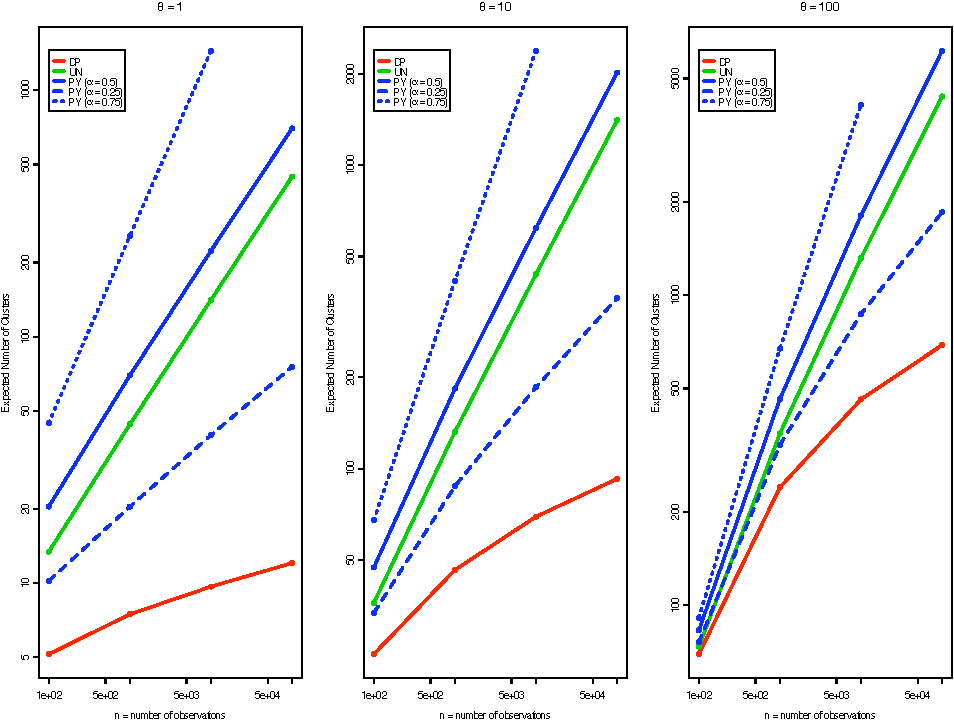
\includegraphics[width=5in,height=2.75in,angle=90]{figures/fig_numberofclusters.pdf}}
\end{center}
\caption{Expected number of clusters $\hat{K}_n$ as a function of
  sample size $n$ for different $\theta$ values.
\comment{ Axes are
on a log scale.}}\label{numberofclusters}
\end{figure*}

\subsection{${\rm E}\,(K_n)$ and ${\rm E}\,(C_{j,n})$ for the Pitman-Yor
  process prediction rule} \label{PY_asymptotic}

Suppose $0 < \alpha < 1$ and $X_1,\ldots, X_n$ are generated using the
Pitman-Yor prediction rule.  \cite{Pit02} demonstrates that as $n \to
\infty$, we have
\begin{equation}
{\rm E}\,(K_n \g{\rm PY}) \approx \frac{\Gamma(1 + \theta)}{
  \alpha\Gamma(\alpha +
\theta)} \cdot  n^{\alpha} \label{PYmom2}
\end{equation}
Pitman's results \cite{Pit02} can also be used to derive the
following result for the distribution of cluster sizes $\bC_n$:
\begin{equation}
{\rm E}\,(C_{j,n} \g{\rm PY}) \approx \frac{\Gamma(1 +
  \theta) \prod_{i=1}^{j-1} (i - \alpha)}{\Gamma(\alpha +
\theta)\,  j !} \cdot n^{\alpha}  \label{PYmom4}
\end{equation}
for every cluster size $j = 1, 2,\ldots,n$.

\subsection{${\rm E}\,(K_n)$ and ${\rm E}\,(C_{j,n})$ for the uniform process
  prediction rule} \label{UN_asymptotic}

The previous literature is far more sparse with regards to the uniform
process prediction rule.  \cite{DicJen08} provide the following result for the
expected number of clusters $K_n$ as $n \to \infty$:
\begin{equation}
{\rm E}\,(K_n\g{\rm UN}) \approx \sqrt{2 \theta} \cdot
n^{\frac{1}{2}} \label{UNmom2}
\end{equation}
In Section~\ref{simulationstudy}, we present simulation-based results
that suggest
the following result for the expectation of cluster sizes $\bC_n$
under the uniform prediction rule:
\begin{equation}
{\rm E}\,(C_{j,n} \g {\rm UN}) \approx \theta.   \qquad
\hbox{as} \,\, n \to \infty 
\ldots \label{UNmom4}
\end{equation}
for every $j = 1, 2,\ldots,n$.  This results fits nicely with the
underlying intuition of the uniform prediction rule, that new
observations are equally likely to join any of the previously existing
clusters, regardless of size.

\subsection{Summary of Asymptotic Results}

To summarize these results, the expected number of clusters $K_n$
grows logarithmically with the sample size under a Dirichlet process
prediction rule, whereas the uniform prediction rule leads the
expected number of clusters $K_n$ to grow with the square root of the
sample size.  Interestingly, the Pitman-Yor prediction rule implies
that the expected number of clusters grows at a rate of $n^\alpha$,
which means that depending on the value of the additional parameter
$\alpha$, the Pitman-Yor prediction rule can lead to a slower or
faster growth rate for $K_n$ than the uniform prediction rule.  For
$\alpha = 0.5$, the expected number of clusters grows at the same rate
for the Pitman-Yor and uniform prediction rules.

The distribution of cluster sizes $\bC_n$ for the uniform rule is
clearly quite different from that of the Pitman-Yor and Dirichlet
processes, as seen in the results above as well as our simulation-based
results in Section~\ref{simulationstudy} below.  In fact, the
distribution of cluster sizes $\bC_n$ for the Pitman-Yor prediction
rule show similar characteristics to $\bC_n$ from the Dirichlet
process prediction rules, despite the closer similarity between the
Pitman-Yor and uniform prediction rules with respect to the number of
clusters $K_n$.  The Pitman-Yor process
can be configured to look similar to a uniform process in terms of the
expected number of clusters, but not in terms of the uniform
distribution of cluster sizes, which is a unique aspect of the uniform
process.

\begin{figure*}[ht]
\begin{center}
\rotatebox{270}{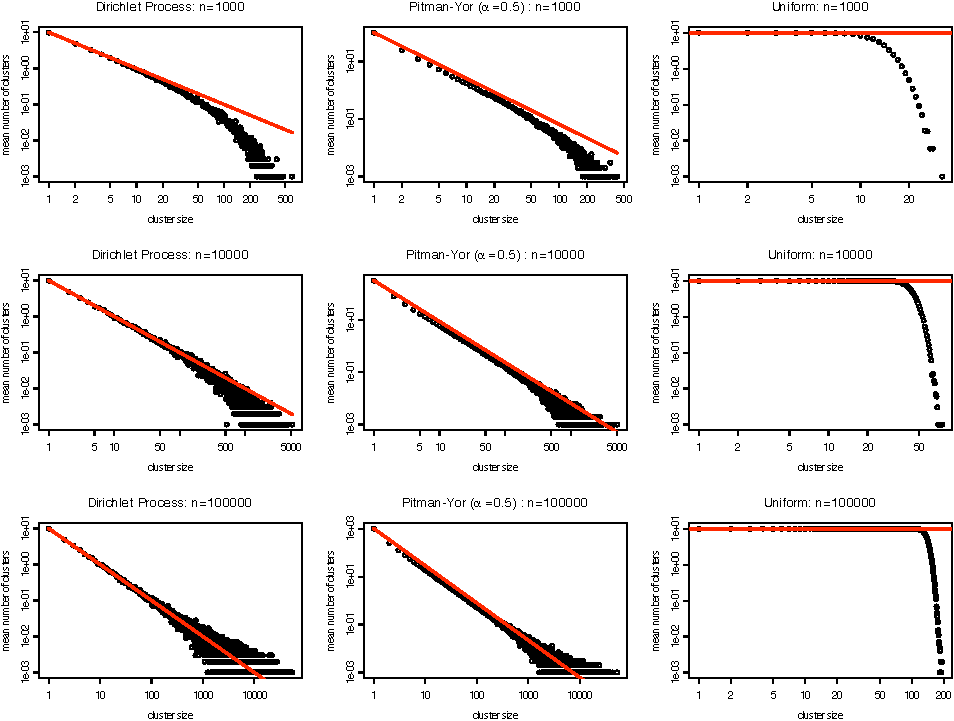
\includegraphics[width=5.5in,height=2.75in,angle=90]{figures/fig_clustersizes.pdf}}
\end{center}
\caption{Cluster sizes $C_{j,n}$ as a function of
  $j$ for different values of $n$ and different prediction rules.   Data is plotted on a log-log
  scale and the red lines in each plot is the relationships suggested
  by our asymptotic results.}\label{simclustersizes}
\end{figure*}

\section{Simulation Comparisons for Finite $n$}\label{simulationstudy}

The asymptotic results presented in the previous section are not
necessarily applicable to finite sample (i.e., $n$ is finite)
where the distribution of cluster sizes is more sensitive to the fact
that the finite number of observations constrains the distribution of
cluster sizes, $\sum_{j} j \cdot C_{j,n} = n$.  We can appraise the
consequences of the three prediction rules in finite samples via a
simulation study.  For various values of sample size $n$ and concentration parameter $\theta$ and for each
of the Dirichlet process, Pitman-Yor and uniform prediction rules, we simulated 1000 independent partitions, and
calculated their corresponding number of clusters $K_n$ and
distribution of cluster sizes $\bC_n$.

\subsection{Comparison of Number of Clusters $K_n$ Between Prediction
  Rules}

In Figure~\ref{numberofclusters}, we examine the relationship between
the number of observations $n$ and the average number of clusters
$\hat{K}_n$ (averaged over the 1000 simulated partitions). We see that
the rate of growth of $\hat{K}_n$ is the same for the uniform and the
Pitman-Yor ($\alpha = 0.5$) prediction rules, which agrees with the
equality suggested by (\ref{PYmom2}) and (\ref{UNmom2}) when $\alpha =
0.5$.  Also, as postulated in Section~\ref{PY_asymptotic}, we see that
depending on the value of $\alpha$, the Pitman-Yor prediction rule can
show either slower ($\alpha=0.25$) or faster ($\alpha=0.75$) rates of
growth of $\hat{K}_n$ compared to the uniform prediction rule.  The
rate of growth of $\hat{K}_n$ for the Dirichlet process prediction
rule is slower than any of the other processes, as suggested by the
logarithmic rate in (\ref{DPmom2}).

\subsection{Comparison of Distribution of Cluster Sizes between
  prediction rules}

We now examine the estimated distribution of cluster sizes $C_{j,n}$
under each prediction rule. For brevity, we focus on $\theta = 10$
only, though the same trends are observed for other values of concentration parameter
$\theta$.  Figure~\ref{simclustersizes} is a plot of $C_{j,n}$, the
number of clusters of size $j$, as a function of $j$.  $C_{j,n}$ was
calculated as the average over the 1000 simulated independent
partitions of $C_{j,n}$ under the three different prediction
rules. The red line in each of the plots is the relationship suggested by our
asymptotic results, i.e., (\ref{DPmom1}) for the Dirichlet process,
(\ref{PYmom4}) for the Pitman-Yor process, and (\ref{UNmom4}) for the
uniform process.

The primary observation from Figure~\ref{simclustersizes} is that the
simulated distribution of the cluster sizes from the uniform process
is quite different to the cluster size distributions generated by
either the Dirichlet process or Pitman-Yor process, as suggested by
the asymptotic results in Section~\ref{asymptotics}.  It is also
interesting to observe the divergence from the asymptotic
relationships due to the finite sample size constraint, especially in
the case of smaller sample sizes ($n = 1000$).

\section{Application to Document Clustering}\label{application}

In this section, we compare the Dirichlet and uniform processes
on the task of clustering documents.  Our specific application consists of 1200 carbon nanotechnology patent abstracts.  Dirichlet processes have been
used as the basis of many document clustering models including those
of~\cite{ZhaGhaYan05},~\cite{ZhuGhaLaf05} and~\cite{Wal08}. In practice, however, it is often the
case in these tasks that there is no reason to justify the \emph{a priori}
``rich-get-richer'' property exhibited by the Dirichlet process.

\begin{figure}[t]
{\hfill
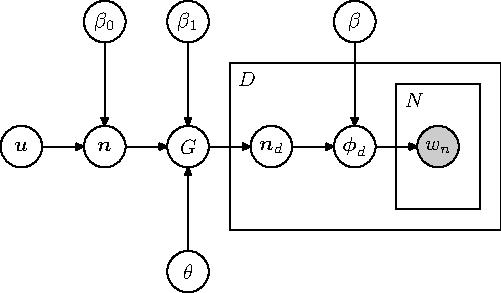
\includegraphics[scale=0.8]{figures/dpmm_fixed-1.pdf}
\hfill}
\caption{Word-based mixture model. $G$ is either drawn from a
  Dirichlet process or a uniform process. Variables $\bn$, $\bu$,
  $\beta_1$ and $\beta_0$ comprise base measure $G_0$.}
\label{fig:dpmm}
\end{figure}

Here, we consider a nonparametric word-based mixture model
(depicted in Figure~\ref{fig:dpmm}), where documents are clustered on
the basis of word occurrences. The model assumes the following
generative process: the tokens $\bw_d$ that comprise each document $d$
are drawn from a document-specific distribution over words $\bphi_d$,
which is itself drawn from a document-specific Dirichlet distribution
with base measure $\bn_d$ and concentration parameter $\beta$. Each
$\bn_d$ is distributed as
\begin{equation}
P(\bn_d \g G) = G(\bn_d)
\end{equation}
where
\begin{equation}
P(G \g \theta, G_0) = \textrm{DP}\,(G \g \theta, G_0) \textrm{ or } \textrm{UP}\,(G \g
\theta, G_0).
\end{equation}
$G$ is is a random probability measure distributed according to either
a Dirichlet or uniform process with base measure $G_0$ and
concentration parameter $\theta$. 

Finally, the base measure $G_0$ is chosen to be a hierarchical
Dirichlet distribution: $G_0 = \textrm{Dir}\,(\bn_{c} \g \beta_1
\bn)$, where $\bn \sim \textrm{Dir}\,(\bn \g \beta_0 \bu)$. This model
captures the fact that documents in different clusters will likely 
use different vocabularies, while allowing each document's word
distribution to vary slightly from the word distribution for the
cluster to which that document belongs.    

The key consequence of using either a Dirichlet or uniform process
prior is that the latent variables $\bn_d$ are partitioned into $C$
clusters where $C$ does not have to be pre-specified.  Let $\bc$ be
the vector of cluster memberships where $c_d$ indicates the cluster
for document $d$.  Given observed documents $\mathcal{W} = \{\bw_d
\}_{d=1}^D$, we can use Gibbs sampling to
iteratively sample the latent cluster memberships $\bc$.
Specifically, the cluster assignment $c_d$ for document $d$ is
resampled from
\begin{align}
&p(c_d \g \bc_{\setminus d}, \bw, \theta) \propto \notag\\
&\qquad p(c_d \g \bc_{\setminus d}, \theta) \, \cdot \, p(\bw_d \g c_d,
\bc_{\setminus d}, \mathcal{W}_{\setminus d}, \bbeta),\label{gibbssampling}
\end{align}
where $\bc_{\setminus d}$ and $\mathcal{W}_{\setminus d}$ denote the
set of clusters and documents, respectively, excluding document $d$.
The vector $\bbeta = (\beta, \beta_1, \beta_0)$ represents the other parameters
in the model, which can be inferred using slice
sampling~\cite{neal03slice}, as described by~\cite{Wal08}.

The likelihood component of (\ref{gibbssampling}) is 
\begin{align}
&p(\bw_d \g c_d,
\bc_{\setminus d}, \mathcal{W}_{\setminus d}, \bbeta)\notag\\
%&=
%\prod_{\{ n \g d_n = d\}} p(w_n \g c_d, \bw_{d}^{(<n)}, \mathcal{W}_{\setminus d}, \bc_{\setminus
%  d}, \bbeta)\\
&= \prod_{\{ n \g d_n = d\}} \frac{N_{w_n|d}^{(<n)} + \beta\,
  \frac{N_{w_n|c_d}^{(<n)} + \beta_1\, \frac{N_{w_n}^{(<n)} + \beta_0\,
      \frac{1}{W}}{\sum_w N_w^{(<n)} + \beta_0}}{\sum_w N_{w|c_d}^{(<n)} +
    \beta_1}}{\sum_w N_{w|d}^{(<n)} + \beta},
\end{align}
where $N_{w|d}^{(<n)}$ is the number of times word type $w$ occurs in
document $d$ (excluding position $n$ onwards), $N_{w|c_d}^{(<n)}$ is
the number of times $w$ occurs in cluster $c_d$ (excluding position
$n$ onwards for document $d$), and $N_w^{(<n)}$ is the number of times
$w$ occurs in the entire corpus (excluding position $n$ onwards for
document $d$).

The conditional prior probability $P(c_d \g \bc_{\setminus d},
\theta)$ is given by any of our discussed prediction rules.  For the sake of brevity, we exclude the Pitman-Yor process and focus our comparisons on the Dirichlet process versus the uniform process.  For the Dirichlet process, we have
\begin{equation}
p(c_d \g \bc_{\setminus d}, \theta)  \propto \begin{cases}
          N_{c_d} & c_d \textrm{ is an
    existing
    cluster}\\
          \theta  & c_d \textrm{ is a new cluster} \end{cases}
\end{equation}
where $N_{c_d}$ is the number of clusters in cluster $c_d$.  For the uniform process we have
\begin{equation}
p(c_d \g \bc_{\setminus d}, \theta)  \propto \begin{cases}
          1 & c_d \textrm{ is an
    existing
    cluster}\\
          \theta  & c_d \textrm{ is a new cluster} \end{cases}
\end{equation}

We compare the Dirichlet process and uniform process priors by using
the model to cluster carbon nanotechnology patents.   For each prior, we
use Gibbs sampling and slice sampling to infer cluster assignments
$\bc^{\textrm{tr}}$ and $\bbeta$ for a set $\mathcal{W}^{\textrm{tr}}$ of 1000 patent
abstracts. To provide insight into the role of concentration parameter $\theta$, we do not allow 
$\theta$ to vary, but instead compare clustering models for several fixed $\theta$ values. We
evaluate predictive performance using a test set $\mathcal{W}$ of 200
patent abstracts and computing the probability of this test set given our trained model.  Specifically, we compute $P(\mathcal{W} \g \mathcal{D}^{\textrm{tr}}, \theta, \bbeta) = \sum_{\bc} P(\mathcal{W}, \bc \g
\mathcal{D}^{\textrm{tr}}, \theta, \bbeta)$, where
$\mathcal{D}^{\textrm{tr}} = (\mathcal{W}^{\textrm{tr}}, \bc^{\textrm{tr}})$ where this sum over test cluster
assignments $\bc$ is approximated using a novel variant of the ``left-to-right''
evaluation algorithm given in Appendix~\ref{leftright}.  

In the left-hand plot of Figure~\ref{resultsfig}, we compare the Dirichlet process to the uniform process in terms of our evaluation metric, $P(\mathcal{W} \g \mathcal{D}^{\textrm{tr}}, \theta, \bbeta)$, the probability of the test data given the trained model.   Regardless of the value of the concentration parameter $\theta$, the trained model based on the uniform process leads to systematically higher probabilities on the test data than the trained model based on the Dirichlet process.   The uniform process clearly seems to be a substantially better fit to the data in this application.   In the right-hand plot of Figure~\ref{resultsfig}, we compared the uniform and Dirichlet processes in terms of the number of clusters in a representative partition produced by the Gibbs sampler.    We see that the uniform process leads to a greater number of clusters than the Dirichlet process for each value of the concentration parameter $\theta$.  This is not a surprising result given our theoretical results for the {\it a priori}  expected cluster sizes (Section~\ref{asymptotics}) and the fact that the choice of clustering prior is clearly influential on the posterior distribution in this application.  
\begin{figure*}[ht]

\vspace{-0.5cm}

\begin{center}
\rotatebox{270}{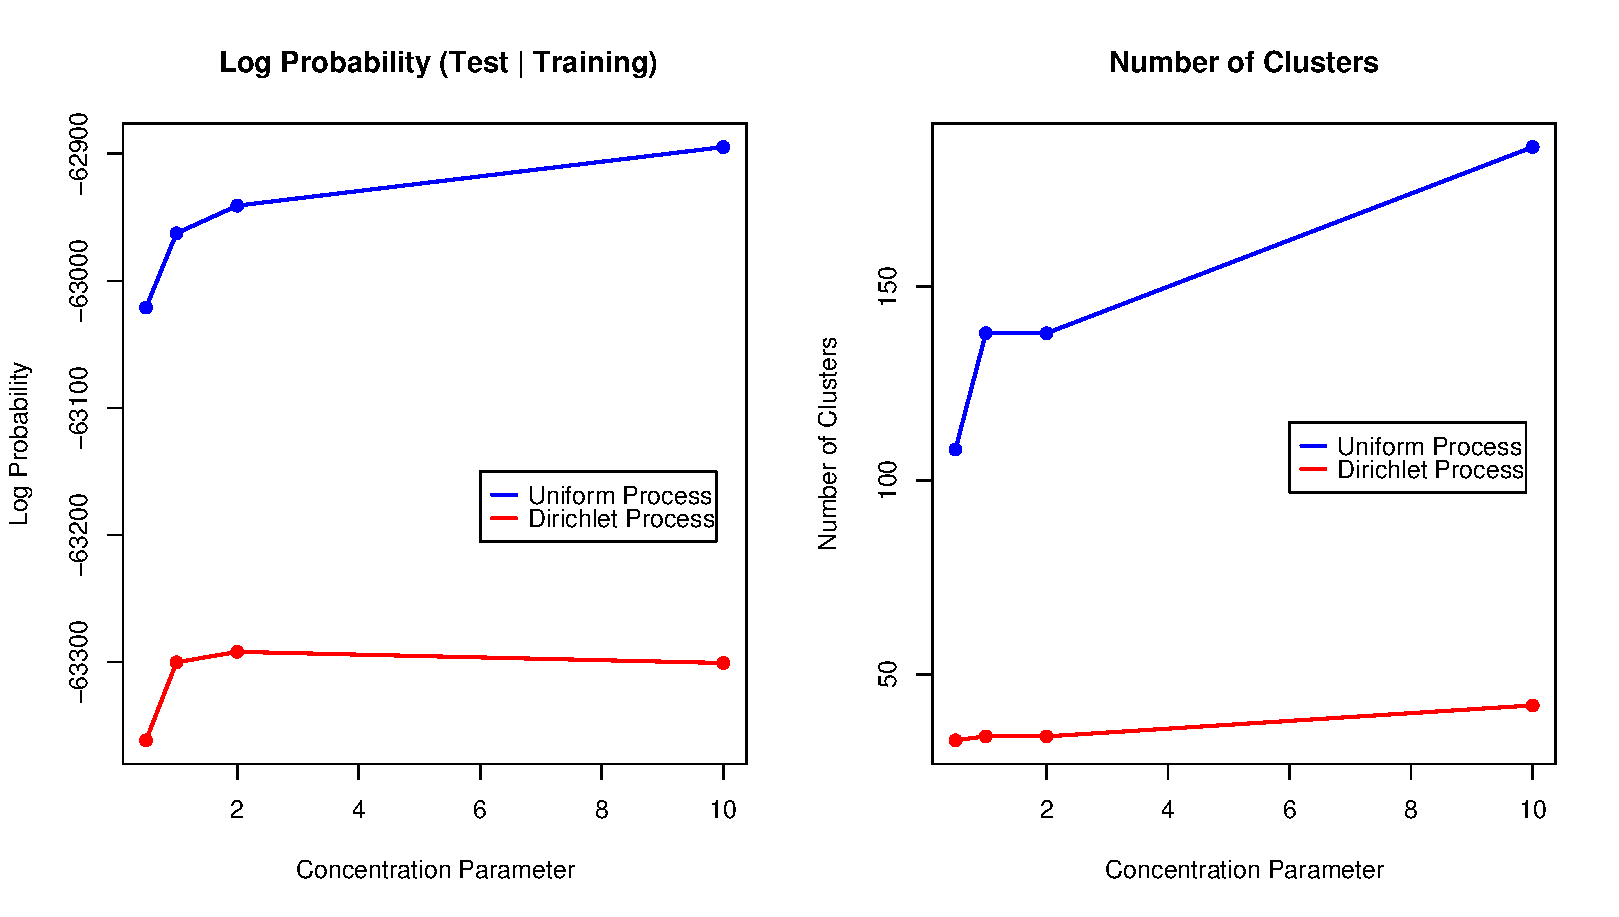
\includegraphics[width=5.5in,height=2.75in,angle=90]{figures/fig_results_combined.pdf}}
\end{center}
\caption{Comparison of the clustering models based on the Dirichlet and uniform processes applied to nanotechnology patent abstracts.  The left plot gives $\log P(\mathcal{W} \g \mathcal{D}^{\textrm{tr}}, \theta, \bbeta)$, the log probability of the test data given the trained model based on either the uniform or Dirichlet process.  The right plot gives the number of clusters in a representative partition from each trained model. }\label{resultsfig}
\end{figure*}



\section{Discussion}\label{discussion}

We have explored and compared the characteristics of three prior
distributions for partitions of random variables.  The popular
Dirichlet process and Pitman-Yor process both have a
``rich-get-richer'' property that leads to partitions with a small
number of relatively large clusters which should be acknowledged by
practitioners when using the Dirichlet process or Pitman-Yor process
within a hierarchical model.  An important consequence of the
``rich-get-richer'' property is that the number of clusters grows
slowly with an
increasing number of observations.  In fact, the expected number of
clusters grows logarithmically as the sample size increases to
infinity in a Dirichlet process.  The Pitman-Yor process 
includes an additional parameter $0 \leq \alpha \leq 1$ that helps to
dampen this ``rich-get-richer'' property.  This parameter $\alpha$
controls the growth of the number of clusters: the expected number of
clusters grows at a rate of $n^\alpha$ as the sample size goes to
infinity.  However, we observed that the distribution of cluster sizes
under the Pitman-Yor process still shows similar characteristics to
the Dirichlet process.

As an alternative to the popular Pitman-Yor and Dirichlet processes,
we have introduced a uniform process prior that eliminates the
preferential attachment property completely.  This uniform process can
be visualized as a ``blindfolded'' version of the popular Chinese
restaurant construction of the Dirichlet process, in the sense that a
customer's decision to join a table is uninfluenced by the size of the
table.  Our simulation studies demonstrate a substantial difference in
the distribution of cluster sizes between the uniform and the
Pitman-Yor or Dirichlet process.  In our application to carbon
nanotechnology patent abstracts, we show superior performance of a
clustering model based on the uniform process compared to the same
clustering model based on the Dirichlet process.

\comment{
\section*{Acknowledgment}

The authors thank Warren Ewens, Dylan Small and David Mimno for many
helpful discussions.
}

\bibliography{references}

\begin{appendix}

\section{Evaluation algorithm} \label{leftright}

Our evaluation is based on the ``left-to-right'' evaluation algorithm introduced by~\cite{Wal08} that has been adapted to
marginalize out test cluster assignments. Pseudocode is given in Algorithm~\ref{alg:particle_lda}.
\begin{algorithm}[ht]
\begin{algorithmic}[1]
{\small
\STATE initialize $l \is 0$
\FOR {each document $d$ in $\mathcal{W}$}
\STATE initialize $p_d \is 0$
\FOR {each particle $r = 1$ to $R$}
\FOR {$d' < d$}
% resample...
\STATE $c^{(r)}_{d'} \sim P(c^{(r)}_{d'} \g \mathcal{W}_{<d},
\{
\bc^{(r)}_{< d} \}_{\setminus
  {d'}}, \mathcal{D}^{\textrm{tr}},,\theta, \bbeta)$
\ENDFOR
\STATE $p_d \is p_d + \sum_c P(\bw_d, c^{(r)}_d \!=\! c \g
\mathcal{W}_{<d},\bc^{(r)}_{<d}, \mathcal{D}^{\textrm{tr}},\theta, \bbeta)$
\STATE $c^{(r)}_d \sim P(c^{(r)}_d \g \bw_d, \mathcal{W}_{<d},\bc^{(r)}_{<d},\mathcal{D}^{\textrm{tr}},\theta,\bbeta)$
\ENDFOR
\STATE $p_n \is p_n \,/\, R$
\STATE $l \is l + \log{p_n}$
\ENDFOR
\STATE $\log{P(\mathcal{W} \g \mathcal{D}^{\textrm{tr}}, \theta, \bbeta)} \simeq l$
}
\end{algorithmic}
\caption{A ``left-to-right'' evaluation algorithm.}
\label{alg:particle_lda}
\end{algorithm}

\end{appendix}

\end{document} 



